\documentclass[
  final,
  babelLanguage=portuguese,
  %desktopVersion,
  %showtrims,
  %overleaf,
]{anecdote}

\graphicspath{{./assets/photos/300dpi/}}

% Page size: 6x9 inch
% Body text: 10.5 / 15 pt

\usepackage{local}

%% Details of the book
%% ===================

\title{Quatro Nobres Verdades}
\subtitle{}
\author{Ajahn Sumedho}
\publisher{Publicações Sumedhārāma}
\date{2018-07-23}
\editionInfo{\emph{Segunda Edição}, impresso na Malásia, 2019}
\ISBN{000-000-0000-00-0}% TODO update ISBN

% === Metadata ===

\hypersetup{
  pdftitle={\thetitle},
  pdfauthor={\theauthor},
  pdfcopyright={Copyright (C) 2019, \thePublisher},
  pdfsubject={},% TODO subject
  pdfkeywords={},% TODO keywords
  pdflicenseurl={https://creativecommons.org/licenses/by-nc-nd/4.0/},
  pdfcontacturl={},
  pdflang={pt},
}

% FIXME macro missing from LuaTeX 2018
%\pdfinfo{%
%  /Title (\thetitle)%
%  /Author (\theauthor)
%  /Subject (subject)% TODO subject
%  /Keywords (keywords)% TODO keywords
%  /GTS_PDFXVersion (PDF/X-1:2001)%
%  /GTS_PDFXConformance (PDF/X-1a:2001)%
%}

%% === Load further packages ===

%% === Hyphenation exceptions and corrections ===

\hyphenation{London}

\begin{document}

\frontmatter

\ifdesktopversion
\desktopCover{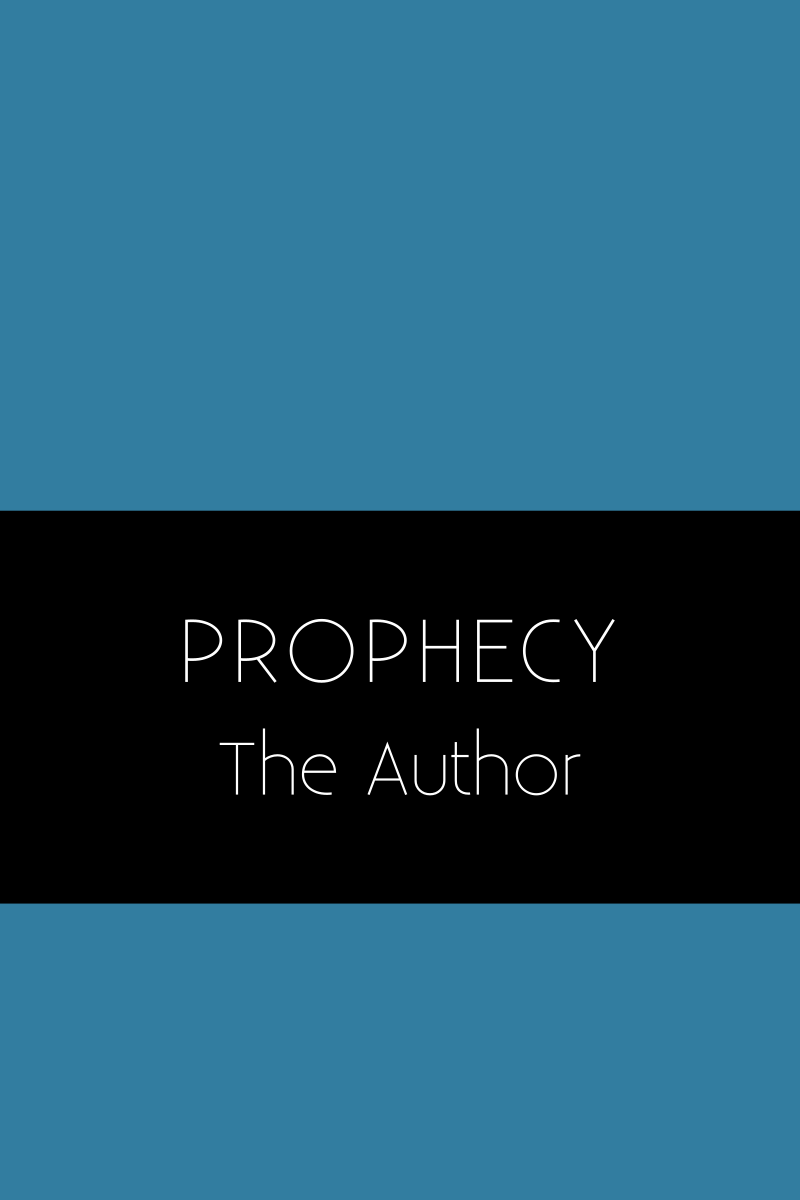
\includegraphics[height=\paperheight]{./desktop-cover.png}}
\fi

\cleartorecto
\thispagestyle{empty}
\vspace*{5em}

{\centering

\settowidth{\titleLength}{%
  {\Large\crimsonRomanFont\scshape\thetitle}%
}

{\Large\crimsonRomanFont\scshape\thetitle}\\[0.3\baselineskip]
\setlength{\xheight}{\heightof{X}}
\raisebox{0.5\xheight}{\color[gray]{0.4}\rule{\titleLength}{0.25pt}}\\[0.3\baselineskip]
{\itshape
\thesubtitle}

\vfill

\theauthor

\vspace*{5em}

}



\cleartoverso
\thispagestyle{empty}

{\copyrightsize
\centering
\setlength{\parindent}{0pt}%
\setlength{\parskip}{0.8\baselineskip}%

\thetitle\ -- \thesubtitle\\
by \theauthor

Published by \thePublisher

ISBN \theISBN

Copyright \copyright\ \thePublisher\ 2017

Cover Photograph: The Person

\vfill

{\footnotesize

This work is licensed under a Creative Commons\\
Attribution-NonCommercial-NoDerivatives 4.0 International~License.

Produced with the \LaTeX\ typesetting system, set in Gentium and Crimson Roman.

\theEditionInfo

}}


\cleartorecto
\thispagestyle{empty}

\mbox{}\vfill

\begin{verse}
\centering
Dedicação

\bigskip

Gostaríamos de deixar o nosso agradecimento a todos aqueles que
contribuíram para a preparação deste livro, e em particular ao grupo
Kataññuta da Malásia, Singapura e Austrália por tornar possível esta~publicação.

\sectionBreak

Dedicado também com gratidão aos meus pais. E à
saudosa memória de minha avó Elisa, que ela possa realizar a
paz do Nibbāna.

Kāñcano Bhikkhu

\end{verse}

\vfill\mbox{}


\cleartorecto
\tableofcontents*

\chapter{Foreword}

Nullam eu ante vel est convallis dignissim. Fusce suscipit, wisi nec facilisis
facilisis, est dui fermentum leo, quis tempor ligula erat quis odio. Nunc porta
vulputate tellus. Nunc rutrum turpis sed pede. Sed bibendum. Aliquam posuere.
Nunc aliquet, augue nec adipiscing interdum, lacus tellus malesuada massa, quis
varius mi purus non odio. Pellentesque condimentum, magna ut suscipit hendrerit,
ipsum augue ornare nulla, non luctus diam neque sit amet urna. Curabitur
vulputate vestibulum lorem. Fusce sagittis, libero non molestie mollis, magna
orci ultrices dolor, at vulputate neque nulla lacinia eros. Sed id ligula quis
est convallis tempor. Curabitur lacinia pulvinar nibh. Nam a sapien.

\bigskip

{\raggedleft
  Reviewer Person\\
  July 2017
\par}


\chapter{Prefácio}

\thispagestyle{bottomcenter}

Este livro foi compilado e editado a partir de palestras proferidas pelo
Venerável Ajahn Sumedho sobre o ensinamento essencial do Buddha - que a
infelicidade humana pode ser transcendida através do caminho espiritual.

A primeira exposição das Quatro Nobres Verdades foi apresentada pelo Buddha, em
528 a.C., no Parque dos Cervos em Sarnāth, perto de Varanāsi, através do
discurso \emph{Sutta Dhammacakkappavattana} – que literalmente
significa “o discurso que coloca em movimento o veículo do ensinamento”.
Excertos deste \emph{sutta} são citados no início de cada capítulo, descrevendo
as Quatro Nobres Verdades. Cada referência corresponde à secção dos livros das
escrituras (Pāli Cânon), onde este discurso pode ser encontrado. No entanto, nas
escrituras, o tema das Quatro Nobres Verdades repete"-se algumas vezes, como por
exemplo na citação que aparece no início da Introdução.

Em muitas das suas palestras Ajahn Sumedho usa a expressão budista de “not"-self”
(\emph{anattā}) “não eu”. Ajahn Sumedho ensina que a raiz da ignorância é a
ilusão da existência de um eu. Desta forma, não está a falar de aniquilação ou
da rejeição das qualidades pessoais, mas sim a indicar como o sofrimento
(\emph{dukkha}) surge quando querermos manter esta identificação com o corpo e
com a mente, sendo esta identificação errada aquilo a que a maioria das
pessoas chama de “eu”.

Outro termo usado muitas vezes por Ajahn Sumedho nas suas palestras é
“deathless”, que surge neste livro com alguma frequência. Por não existir em
português uma única palavra que ilustre claramente o seu significado, foi
traduzido de diferentes formas, usando"-se os termos que melhor se adequavam ao
contexto de cada situação. Podemos ainda acrescentar que a palavra se refere,
não ao sentido de imortalidade mas sim àquilo que está para além do ciclo de
vida e de morte, não em termos metafísicos mas sim no sentido de impermanência -
“Tudo o que surge está sujeito a cessar” – não se tratando portanto da
derradeira realidade. Nas escrituras existe uma passagem que pode ajudar a
clarificar um pouco mais a palavra “deathless”:

\begin{quote}
  «Existe, bhikkhus, um não nascido, não formado, incriado, o originado. 
  Se não existisse este não nascido, não formado, incriado, não
  originado, não existiria o nascido, o formado, o criado e o originado. Porém,
  precisamente porque existe um não nascido, não formado, incriado e não
  originado, é possível a libertação do nascido, formado, criado e originado».

  \quoteRef{Nibbāna Sutta, Ud 8.3}
\end{quote}

Luang Por Sumedho oferece"-nos a seguinte reflexão sobre esta profunda
declaração: «Podemos ver que não somos vítimas prisioneiras da condição do
nascimento, sem qualquer esperança de escaparmos ao sofrimento da mudança, dos
nossos hábitos e desejos. Existe, assim, uma saída: realizar a existência do não
nascido, não formado, incriado, não originado. Reconhecer, isso é \emph{sati
  sampajaññā}, \emph{sati paññā} ou consciência.

É perceber a diferença entre
estar e não estar apegado à forma, ao que é criado. Nibbāna é a realidade do
não"-apego aos fenómenos condicionantes; não se trata de destruir o
\emph{saṃsāra}, de aniquilar todos as condições por estas serem tão limitadoras
e só conduzirem ao sofrimento, mas sim de reconhecer e discernir essa realidade».

Concluindo, estas Quatro Nobres Verdades são como que um exercício de
discernimento; ajudam a não tomar posições rígidas a favor ou contra o que quer
que seja, mas sim a reconhecer o Não Nascido e Não Criado como verdadeiro, e não
como uma fantasia ou um ideal. Desta forma, esta realidade é reconhecida e
cultivada na nossa vida quotidiana.

Caro leitor, o desejo é que, ao explorar as seguintes páginas, os corações de
todos aqueles que tiveram a oportunidade de encontrar a sabedoria dos
ensinamentos aqui contidos, se sintam inspirados a despertar, e rapidamente
realizem o fim de todo o sofrimento.

\bigskip

{\raggedleft
  Kāñcano Bhikkhu\\
  Mosteiro Amarāvatī\\
  Outubro 2007
\par}



% Page 1 is the first page of the first chapter.
\mainmatter

\chapterNote{Chapter one subtitle}

\chapter{Chapter One Title}
\tocChapterNote{Chapter one subtitle}

Aliquam erat volutpat. Nunc eleifend leo vitae magna. In id erat non orci
commodo lobortis. Proin neque massa, cursus ut, gravida ut, lobortis eget,
lacus. Sed diam. Praesent fermentum tempor tellus. Nullam tempus. Mauris ac
felis vel velit tristique imperdiet. Donec at pede. Etiam vel neque nec dui
dignissim bibendum. Vivamus id enim. Phasellus neque orci, porta a, aliquet
quis, semper a, massa. Phasellus purus. Pellentesque tristique imperdiet tortor.
Nam euismod tellus id erat.


\chapterNote{Chapter two subtitle}

\chapter{Chapter Two Title}
\tocChapterNote{Chapter two subtitle}

Nullam eu ante vel est convallis dignissim. Fusce suscipit, wisi nec facilisis
facilisis, est dui fermentum leo, quis tempor ligula erat quis odio. Nunc porta
vulputate tellus. Nunc rutrum turpis sed pede. Sed bibendum. Aliquam posuere.
Nunc aliquet, augue nec adipiscing interdum, lacus tellus malesuada massa, quis
varius mi purus non odio. Pellentesque condimentum, magna ut suscipit hendrerit,
ipsum augue ornare nulla, non luctus diam neque sit amet urna. Curabitur
vulputate vestibulum lorem. Fusce sagittis, libero non molestie mollis, magna
orci ultrices dolor, at vulputate neque nulla lacinia eros. Sed id ligula quis
est convallis tempor. Curabitur lacinia pulvinar nibh. Nam a sapien.




\backmatter

\chapter{Glossário}

\begin{glossarydescription}

% === A ===

\item[Ajahn] (Thai) palavra Tailandesa para mestre, mentor, professor;
  frequentemente usada como titulo para monges seniores. Palavra equivalente ao
  Pāli “ācariya”.

% === B ===

\item[Bhikkhu] (Pāli) mendicante; termo para o monge budista que vive das
  ofertas e assume os preceitos de treino que definem a vida de renúncia e
  moralidade.

\item[Buddha-rūpa] (Pāli) Corpo do Buddha ou Bodhi.

% === C ===

% === D ===

\item[Dhamma] (Pāli; em Sânscrito: \emph{Dharma}) esta palavra tem vários
  significados, tais como dever, a lei da verdade universal, a natureza ou
  constituição das coisas, lei, norma, objecto da mente, fenómenos ou princípios
  de comportamentos que ao serem seguidos integram os seres humanos na ordem
  natural das coisas; qualidades da mente a ser desenvolvidas para se poder
  compreender a qualidade da mente em si mesma. Nos textos a palavra é
  encontrada com todos estes significados. Dhamma refere-se tanto aos
  ensinamentos do Buddha contidos nas escrituras, como à experiência directa da
  verdade suprema para a qual os seus ensinamentos são direccionados.

\item[Dia de Observância] (em Pāli: \emph{Uposatha}) um dia sagrado ou
  “sabbath”, ocorre em todos dias de Lua Nova e Lua Cheia. Nestes dias os
  budistas reúnem-se para ouvir o Dhamma e reafirmam a sua prática em termos de
  preceitos e meditação.

% === E ===

% === F ===

% === G ===

% === H ===

% === I ===

% === J ===

% === K ===

\item[Kamma] (Pāli; em Sânscrito: \emph{karma}) Acção de causa e efeito. Causa que é
  criada e recriada pelos impulsos habituais, vontade própria ou energias
  naturais. Manifesta-se de forma benéfica ou prejudicial no corpo, na linguagem
  e na mente. Marcas ou impressões que ficam na nossa mente causando o
  renascimento e moldando o destino dos seres. Este termo, popularmente usado,
  inclui também o sentido de resultado ou efeito da acção, embora o termo
  correcto para isto seja vipāka.

% === L ===

% === M ===

% === N ===

% === O ===

% === P ===

\item[Paṭicca-samuppāda] (Pāli) origem dependente, a apresentação por etapas de
  como o sofrimento surge dependendo do grau de ignorância e de desejo e, de
  como termina com a sua cessação.

% === Q ===

% === R ===

% === S ===

% === T ===

\item[Tipiṭaka] (Pāli) literalmente “três cestos”, a colecção das escrituras
  Budistas, classificadas de acordo com Sutta (Discursos), Vināya (Disciplina ou
  Treino) e Abhidhamma (Metafísica).

% === U ===

% === V ===

\item[Vipassanā] (Pāli) significa ver a verdadeira natureza das coisas, na sua
  realidade. É um processo de auto-transformação através da auto-observação. Um
  método analítico baseado na atenção plena, vigilância e investigação dos
  fenómenos manifestados nos cinco agregados “\emph{khandha}”, nomeadamente
  forma física “\emph{rūpa}”, sensações ou sentimentos “\emph{vedanā}”,
  percepção “\emph{saññā}”, formações mentais “\emph{saṅkhāra}” e consciência
  “\emph{viññāṇa}”.

% === W ===

\end{glossarydescription}



\cleartorecto
\thispagestyle{plain}
\vspace*{-2.5\baselineskip}%

\enlargethispage{\baselineskip}

{\fontsize{9}{10.5}\selectfont\setlength{\parindent}{0pt}%
\raggedright\label{copyright-details}
\setlength{\parskip}{4.5pt}

{\centering

{\LARGE\ccbyncnd}

\vspace*{0.5\onelineskip}

Este trabalho está licenciado com uma Licença Creative Commons\\
Atribuição-NãoComercial-SemDerivações 4.0 Internacional.\footnote{%
\href{http://creativecommons.org/licenses/by-nc-nd/4.0/deed.pt}{http://creativecommons.org/licenses/by-nc-nd/4.0/deed.pt}}

}

Você tem o direito de:

\begin{packeditemize}
\item Compartilhar — copiar e redistribuir o material em qualquer suporte ou formato
\end{packeditemize}

O licenciante não pode revogar estes direitos desde que respeite os termos da licença.

De acordo com os termos seguintes:

\begin{packeditemize}
\item Atribuição — Deve atribuir o devido crédito, fornecer um link para a licença, e indicar se foram feitas alterações. Pode fazê-lo de qualquer forma razoável, mas não de uma forma que sugira que o licenciante o apoia ou aprova o seu uso.
\item NãoComercial — Não pode usar o material para fins comerciais.
\item SemDerivações — Se reestruturar, transformar, ou criar a partir do material, não pode distribuir o material modificado.
\end{packeditemize}

Sem restrições adicionais — Não pode aplicar termos jurídicos ou medidas de caráter tecnológico que restrinjam legalmente outros de fazerem algo que a licença permita.

Avisos:

Não tem de cumprir com os termos da licença relativamente a elementos do material que estejam no domínio público ou cuja utilização seja permitida por uma expceção ou limitação que seja aplicável.

Não são dadas quaisquer garantias. A licença pode não lhe dar todas as autorizações necessárias para o uso pretendido. Por exemplo, outros direitos, tais como direitos de imagem, de privacidade ou direitos morais, podem limitar o uso do material.

As Publicações Sumedhārāma são parte do `Budismo Theravada da Floresta -- Comunidade Religiosa', uma Pessoa Colectiva Religiosa registada em Portugal com o NIPC 592010040.

O `Budismo Theravada da Floresta -- Comunidade Religiosa', actuando como Publicações Sumedhārāma, reclama o direito moral de ser identificado como o autor deste livro.

O `Budismo Theravada da Floresta -- Comunidade Religiosa', requer que seja atribuída a autoria deste trabalho às Publicações Sumedhārāma sempre que este for reproduzido, distribuído, apresentado ou representado.

}


\emptyUntilModEight

\end{document}
